% This is text associated with the open textbook "Open Electromagnetics"
% See immediately below for author, date
% This work is licensed under the Creative Commons Attribution-ShareAlike 4.0 International License. (CC BY-SA 4.0) 
% To view a copy of the license, visit http://creativecommons.org/licenses/by-sa/4.0/

%ORB TITLE The Thin Parallel Plate Capacitor
%ORB AUTHOR 0        # S.W. Ellingson, Virginia Tech (ellingson@vt.edu)
%ORB DATE 20180806   # yyyymmdd
%ORB ABSTRACT Thin parallel plate capacitor

\label{m0070_Parallel_Plate_Capacitor_Capacitance_from_Charge} % <-- Must match name of this file and module directory name.  Don't mess with this!
\index{capacitor!parallel plate|(}

Let us now determine the capacitance of a common type of capacitor known as the \emph{thin parallel plate capacitor}, 
shown in Figure~\ref{m0070_fPPCap}.
This capacitor consists of two flat plates, each having area $A$, separated by distance $d$.
To facilitate discussion, let us place the origin of the coordinate system at the center of the lower plate, with the $+z$ axis directed toward the upper plate such that the upper plate lies in the $z=+d$ plane.
%
\begin{figure}[b!]
\begin{center}
\pdftooltip{{  % note double braces
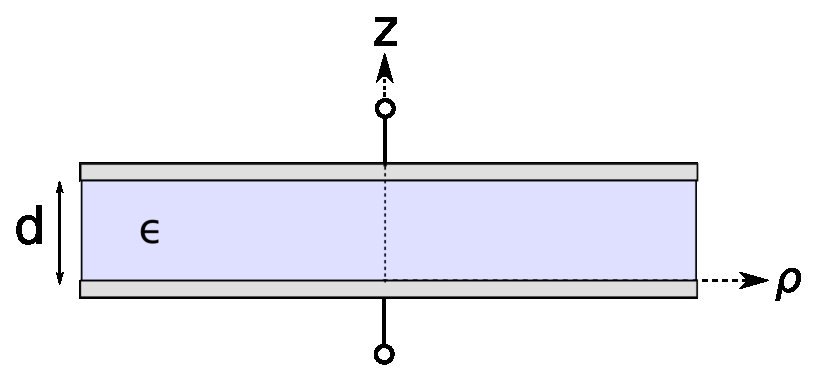
\includegraphics[width=2.5in]{modules/m0070_fPPCap.eps}
%% https://en.wikipedia.org/wiki/File:Parallel_plate_capacitor.svg
}}{A parallel plate capacitor lying horizontal with a node above and below the capacitor drawn on the x-axis similar to a previous figure. The thin plates on top and bottom are represented by silver lines, and the spacer material between colored blue and labeled epsilon. The distance between the plates is labeled d. A dashed arrow points from the z-axis out of the bottom right side of the capacitor, labeled rho.}
\end{center} 
%\centerline{\scriptsize 
%by~\hyperref[m0070_fPPCap_Credit]{inductiveload} (modified)
%%\href{https://creativecommons.org/licenses/by-sa/4.0/}{CC BY-SA 4.0} 
%} 
\caption{
\label{m0070_fPPCap}
Thin parallel plate capacitor.
}
\end{figure}

Below we shall find the capacitance by assuming a particular charge on one plate, using the boundary condition on the electric flux density ${\bf D}$ to relate this charge density to the internal electric field, and then integrating over the electric field between the plates to obtain the potential difference.  Then, capacitance is the ratio of the assumed charge to the resulting potential difference.

The principal difficulty in this approach is finding the electric field. 
To appreciate the problem, first consider that if the area of the plates was infinite, then the electric field would be very simple; it would begin at the positively-charged plate and extend in a perpendicular direction toward the negatively-charged plate (Section~\ref{m0025_Charge_and_Electric_Field_for_a_Perfectly_Conducting_Region}).  Furthermore, the field would be constant everywhere between the plates.  This much is apparent from symmetry alone.
However, when the plate area is finite, then we expect a \emph{fringing field} 
\index{fringing (field)}
to emerge.  ``Fringing field'' is simply a term applied to the non-uniform field that appears near the edge of the plates. The field is non-uniform in this region because the boundary conditions on the \emph{outside} (outward-facing) surfaces of the plates have a significant effect in this region. 
In the central region of the capacitor, however, the field is not much different from the field that exists in the case of infinite plate area.

In any parallel plate capacitor having finite plate area, some fraction of the energy will be stored by the approximately uniform field of the central region, and the rest will be stored in the fringing field.  We can make the latter negligible relative to the former by making the capacitor very ``thin,'' in the sense that the smallest identifiable dimension of the plate is much greater than $d$.  
Under this condition, we may obtain a good approximation of the capacitance by simply neglecting the fringing field, since an insignificant fraction of the energy is stored there.

Imposing the ``thin'' condition leads to three additional simplifications.  
First, the surface charge distribution may be assumed to be approximately uniform over the plate, which greatly simplifies the analysis.
Second, the shape of the plates becomes irrelevant; they might be circular, square, triangular, etc. 
When computing capacitance in the ``thin'' case, only the plate area $A$ is important. 
Third, the thickness of each of the plates becomes irrelevant.

We are now ready to determine the capacitance of the thin parallel plate capacitor.  Here are the steps:
%  
\begin{enumerate}
\item Assume a total positive charge $Q_+$ on the upper plate.
\item Invoking the ``thin'' condition, we assume the charge density on the plates is uniform.  Thus, the surface charge density on bottom side of the upper plate is $\rho_{s,+} = Q_+/A$ (C/m$^2$).  
\item \label{m0070_iStep1} From the boundary condition on the bottom surface of the upper plate, ${\bf D}$ on this surface is $-\hat{\bf z}\rho_{s,+}$. 
\item The total charge on the lower plate, $Q_-$, must be equal and opposite the total charge on the upper plate; i.e, $Q_-=-Q_+$.  Similarly, the surface charge density on the upper surface of the lower plate, $\rho_{s,-}$, must be $-\rho_{s,+}$.
\item 
From the boundary condition on the top surface of the lower plate (Section~\ref{m0021_Boundary_Conditions_on_D}), ${\bf D}$ on this surface is $+\hat{\bf z}\rho_{s,-}$.  
Since $+\hat{\bf z}\rho_{s,-}=-\hat{\bf z}\rho_{s,+}$, ${\bf D}$ on the facing sides of the plates is equal. 
\item Again invoking the ``thin'' condition, we assume ${\bf D}$ between the plates has approximately the same structure as we would see if the plate area was infinite.  Therefore, we are justified in assuming ${\bf D}\approx-\hat{\bf z}\rho_{s,+}$ \emph{everywhere} between the plates.  (You might also see that this is self-evident from the definition of ${\bf D}$ as the flux density of electric charge (Section~\ref{m0011_Electric_Flux_Density}).)
\item With an expression for the electric field in hand, we may now compute the potential difference $V$ between the plates as follows (Section~\ref{m0061_Force_Energy_and_Potential_Difference}):
%
\begin{flalign}
V &= -\int_{\mathcal C}{ {\bf E} \cdot d{\bf l} }  \nonumber \\
  &= -\int_{0}^{d}{ \left(\frac{1}{\epsilon}{\bf D}\right) \cdot \left(\hat{\bf z}dz\right) } \nonumber \\
  &= -\int_{0}^{d}{ \left(-\hat{\bf z}\frac{\rho_{s,+}}{\epsilon}\right) \cdot \left(\hat{\bf z}dz\right) } \nonumber \\
  &= +\frac{\rho_{s,+}~d}{\epsilon}
\end{flalign} 
%
\item Finally,
%
\begin{equation}
C = \frac{Q_+}{V} = \frac{\rho_{s,+}~A}{\rho_{s,+}~d/\epsilon} = \frac{\epsilon A}{d}
\end{equation}
%
\end{enumerate}

Summarizing:
%
\begin{equation}
\boxed{
C \approx \frac{\epsilon A}{d}
}
\label{m0070_eTPPC}
\end{equation}
%
%ORB HIGHLIGHT
\begin{mdframed}[backgroundcolor=yellow!20,nobreak=true] 
The capacitance of a parallel plate capacitor having plate separation much less than the size of the plate is given by Equation~\ref{m0070_eTPPC}.
This is an approximation because the fringing field is neglected. 
\end{mdframed}
%
It's worth noting that this is dimensionally correct; i.e., F/m times m$^2$ divided by m yields F.
It's also worth noting the effect of the various parameters:
%
%ORB HIGHLIGHT
\begin{mdframed}[backgroundcolor=yellow!20,nobreak=true] 
Capacitance increases in proportion to permittivity and plate area and decreases in proportion to distance between the plates.
\end{mdframed}

\index{printed circuit board (PCB)!capacitance|(}
%ORB EXAMPLE
~\\ \begin{example} 
\begin{mdframed}[backgroundcolor=brown!20,linecolor=brown!20]\raggedright
Printed circuit board capacitance. 
\\~\\
Printed circuit boards commonly include a ``ground plane,'' 
\index{ground plane}
which serves as the voltage datum for the board, and at least one ``power plane,'' which is used to distribute a DC supply voltage (See ``Additional Reading'' at the end of this section).  These planes are separated by a dielectric material, and the resulting structure exhibits capacitance.  This capacitance may be viewed as an equivalent discrete capacitor in parallel with the power supply. 
The value of this equivalent capacitor may be either negligible, significant and beneficial, or significant and harmful.  So, it is useful to know the value of this equivalent capacitor.   

For a common type of circuit board, the dielectric thickness is about 1.6~mm and the relative permittivity of the material is about 4.5.  If the area in common between the ground and power planes is 25~cm$^2$, what is the value of the equivalent capacitor?

{\bf Solution.}
From the problem statement, 
$\epsilon\cong 4.5\epsilon_0$, 
$A \cong 25$~cm$^2$ $=$ $2.5~\times 10^{-3}$~m$^2$, and
$d \cong 1.6$~mm.
Using Equation~\ref{m0070_eTPPC}, the value of the equivalent capacitor is $62.3$~pF.

\end{mdframed}\end{example}

\index{printed circuit board (PCB)!capacitance|)}

%%%%%%%%%%%%%%%%%%%%%%%%%%%%%%%%%%%%

{\bf Additional Reading:}
\begin{itemize}
\item ``\href{https://en.wikipedia.org/wiki/Printed_circuit_board}{Printed circuit board}'' on Wikipedia.
\end{itemize}

\index{capacitor!parallel plate|)}
